\chapter{DIFFERENTIALS OF TRIGONOMETRIC FUNCTIONS}
\setcounter{section}{22}

\section{Angle Measure and Angle Functions}

If through the center $O$ of the circle in \autoref{fig:circle_motion} (article 2) we lay off the horizontal line $OX$ of \autoref{fig:straight_line} (article 1), join the points $O$ and $P$, and draw through $O$ the vertical $OY$, we get \autoref{fig:trig_functions}. \autoref{fig:trig_functions} is thus a combination of \autoref{fig:straight_line} and \autoref{fig:circle_motion} and there are differentials to be measured horizontally, vertically and tangentially.

\begin{figure}[h]
    \centering
    \begingroup
    \begin{tikzpicture}[scale=2]
        % Draw coordinate axes
        \draw[->] (-2.5,0) -- (2.5,0) node[right, scale=1.0] {$X$};
        \draw[->] (0,-2.5) -- (0,2.5) node[above, scale=1.0] {$Y$};
        
        % Draw circle with radius a
        \draw (0,0) circle (2);
        \node[above right, scale=1.0] at (2,0) {$M$};  % Add M label at circle intersection
        
        % Draw point P and its construction lines (30 degrees = pi/6)
        \coordinate (P) at ({2*cos(30)},{2*sin(30)});  % at 30 degrees
        \coordinate (T) at ({2*cos(30) - sin(30)},{2*sin(30) + cos(30)});  % end of tangent vector
        
        % Calculate P' position (intersection of OT with circle)
        \coordinate (Pprime) at ({2*cos(60)},{2*sin(60)});  % P' at 60 degrees
        
        % Add point B and its construction
        \coordinate (B) at ({2*cos(30) - sin(30)},{2*sin(30)});  % B is directly below T
        \draw[dashed] (T) -- (B);  % vertical line from T to B
        \draw[dashed] (P) -- (B);  % horizontal line from P to B
        \node[right, scale=1.0, inner sep=1pt] at ({2*cos(30) - 1.0*sin(30)},{2*sin(30) + 0.8*cos(30)}) {$\theta$};  % Label angle BTP
        
        % Draw dashed construction lines
        \draw[dashed] (P) -- ({2*cos(30)},0) node[below, scale=1.0] {$A$};  % vertical projection
        \draw[dashed] (P) -- (Pprime);  % P to P'
        
        % Draw radius OP and tangent line
        \draw (0,0) -- (P);  % radius
        % Tangent line (perpendicular to radius at P, pointing counterclockwise)
        \draw (P) -- (T) node[above, scale=1.0] {$T$};  % tangent line
        
        % Draw dotted line from O to T
        \draw[dotted] (0,0) -- (T);
        
        % Add points and labels
        \node[left, scale=1.0] at (0,0) {$O$};
        \node[right, scale=1.0] at (P) {$P$};
        \node[above, scale=1.0] at (Pprime) {$P'$};
        \node[below left, scale=1.0] at (B) {$B$};  % Label for point B
        
        % Add angle θ and dθ
        \draw (0,0) + (0:0.8) arc (0:30:0.8);  % angle arc for theta
        \node[right, scale=1.0] at (0.5,0.15) {$\theta$};
        
        % Draw angle dθ at O (between OP and OT)
        \draw[thick] (0,0) + (30:1.0) arc (30:56:1.0);  % arc from OP to OT
        \node[left, scale=1.0] at (0.7,0.6) {$d\theta$};
        
        % Add measurement labels
        \node[above, scale=1.0] at ({2*cos(30) - sin(30)/2},{2*sin(30)}) {$dx$};
        \node[left, scale=1.0] at ({2*cos(30) - sin(30)},{2*sin(30) + cos(30)/2}) {$dy$};
        \node[right, scale=1.0] at ({2*cos(30) - sin(30)/2},{2*sin(30) + cos(30)/2}) {$ds$};
        \node[below, scale=1.0] at (1,0) {$x$};
        \node[left, scale=1.0] at ({2*cos(30) - 0.0},0.5) {$y$};
        \node[below right, scale=1.0] at (1,0.5) {$a$};
    \end{tikzpicture}
    \caption{Trigonometric functions and their differentials.}
    \label{fig:trig_functions}
    \endgroup
\end{figure}

Motion measured parallel to $OX$ toward the right is to be taken as positive and toward the left as negative, as in \autoref{fig:straight_line}; similarly motion parallel to $OY$ and upward is positive, downward is negative. Also as in \autoref{fig:circle_motion}, if the point $P$ moves in the direction opposite to that of the end of the hand of a clock (counter clockwise), the differential of length along the tangent $PT$ is taken as positive, the opposite sense (clockwise) as negative.

As in \autoref{fig:straight_line}, horizontal distances are denoted by $x$, similarly vertical distances are denoted by $y$. Distances measured along the circumference of the circle are denoted by $s$ and differentials of $s$, taken along the instantaneous tangent at any point $P$, by $ds$, as in \autoref{fig:circle_motion}.

With the above system of notation $x$, $y$ are then called the coordinates of the point $P$, and if we imagine the point $P$ to move along the tangent line $PT$ with the direction and speed it had at $P$, covering the differential of distance $ds$ in the time $dt$ as in \autoref{fig:circle_motion} the coordinate $y$ will change by the differential amount $dy$ in the positive sense and $x$ will change by $dx$ in the negative sense. If the angle $AOP$ be represented by the symbol $\theta$ (pronounced ``theta'') then as $P$ moves along $PP'$ the radius $OP=a$ will turn about the center $O$ and $\theta$ will increase by the positive differential of angle $d\theta$.

The question we now have to answer is this: When $P$ moves through a space differential $ds$ and the angle $\theta$ changes by the corresponding differential $d\theta$, what are the corresponding differentials of the angle functions of $\theta$, that is, what are the values of the differentials $d(\sin \theta)$, $d(\cos\theta)$, etc.?

Since $\sin \theta$, $\cos \theta$, $\tan \theta$, etc., are functions of the independent variable $\theta$, then as we have already seen their differentials will depend on $d\theta$ and also on some other function of $\theta$ itself. In the present chapter we shall find the formulas giving these differentials.

In order to find the differentials of the angle functions, or angular functions (also called circular and trigonometric functions, for obvious reasons) we need to understand the method of measurement of $\theta$ and $d\theta$.

If the angle is expressed in degree measure, then the unit of angle is such that the arc intercepted on the circumference by a central angle of one degree is equal in length to the 360th part of the circumference. This is the system used in ordinary computation and in the trigonometric tables.

A more convenient system for formulation and analysis is the so-called circular measure, in which the unit of angle is such that the arc intercepted on the circumference by a central angle of one radian is equal in length to the radius of the circle. Then since the entire circumference equals $2\pi$ times the radius, it equals $2\pi$ times the arc of one radian and there are $2\pi$ radians of angle in the circle. Thus, if the radius of the circle is $a$, one radian intercepts an arc of length $a$, and an angle of $\theta$ radians intercepts an arc of $\theta$ times $a$. If, therefore, the point $P$ in \autoref{fig:trig_functions} moves a distance along the circumference of $MP = s$ while the line $OP$ turns through an angle $\theta$ the length of $MP$ is
\begin{equation}
s = a\theta \tag{29}\label{eq:29}
\end{equation}

By the use of the circular measure we have that $360^\circ = 2\pi$ radians, $180^\circ = \pi$ and $90^\circ = \frac{\pi}{2}$, with corresponding conversions for other angles. These values will be found more convenient than the values expressed in degrees, and the formula (\eqref{eq:29}) is a much more convenient formula for the length of an arc than the corresponding formula in which the angle is expressed in degrees. Except for numerical computation in which the trigonometric tables have to be used we shall use circular measure throughout this book.\footnote{A detailed explanation of this system of angle measure is given in the author's ``Trigonometry for the Practical Man,'' published by D. Van Nostrand Company, New York, N.Y.}

\section{Differentials of the Sine and Cosine of an Angle}

In \autoref{fig:trig_functions} we have, by trigonometry, in the right triangle $AOP$,
\[\sin \theta = \frac{y}{a}, \quad \cos \theta = \frac{x}{a},\]
therefore
\begin{equation}
d(\sin\theta) = \frac{dy}{a}, \quad d(\cos\theta) = \frac{dx}{a} \tag{30}\label{eq:30}
\end{equation}
since $a$ is constant. We have also, since $PT$ is a tangent and perpendicular to $OP$, and $BT$ is perpendicular to $OA$, the angle $PTB$ is equal to $\theta$. Therefore in the right triangle $PTB$, by trigonometry,
\[\frac{dy}{ds} = \cos \theta, \quad \frac{-dx}{ds} = \sin \theta,\]
($dx$ being negative in the figure as already pointed out). Hence
\begin{equation}
dy = (\cos \theta)\cdot ds, \quad dx = -(\sin \theta)\cdot ds. \tag{31}\label{eq:31}
\end{equation}

If we now go back to equation (29) and differentiate it by formula (E), $a$ being constant, we get
\[ds = a\,d\theta\]
and this value of $ds$ substituted in the two equations (31) gives
\[dy = (\cos \theta)\cdot a\,d\theta, \quad dx = -(\sin \theta)\cdot a\,d\theta,\]
or
\[\frac{dy}{a} = \cos \theta\cdot d\theta, \quad \frac{dx}{a} = -\sin\theta\cdot d\theta.\]

Substituting these values of $dy/a$ and $dx/a$ in equations (30) we have finally,
\begin{equation}
d(\sin \theta) = \cos \theta\cdot d\theta \tag{M}\label{eq:M}
\end{equation}
\begin{equation}
d(\cos \theta) = -\sin \theta\cdot d\theta \tag{N}\label{eq:N}
\end{equation}

Thus the answer to our question in the preceding article is that the differential of the sine of an angle is the differential of the angle multiplied by the cosine, and the differential of the cosine is the differential of the angle multiplied by the negative of the sine.

From formulas (\eqref{eq:M}) and (\eqref{eq:N}), the rates of the sine and cosine are,
\begin{equation}
\frac{d(\sin \theta)}{dt} = \cos \theta\cdot\frac{d\theta}{dt}, \quad \frac{d(\cos \theta)}{dt} = -\sin \theta\cdot\frac{d\theta}{dt} \tag{32}\label{eq:32}
\end{equation}
and the derivatives with respect to $\theta$ are,
\begin{equation}
\frac{d(\sin \theta)}{d\theta} = \cos \theta, \quad \frac{d(\cos \theta)}{d\theta} = -\sin \theta \tag{33}\label{eq:33}
\end{equation}

\section{Differentials of the Tangent and Cotangent of an Angle}

The differential of the tangent is found by applying the fraction formula (K) to the following expression, which is obtained from trigonometry:
\[\tan \theta = \frac{\sin \theta}{\cos \theta}\]

Differentiating this by the formula (K) we get
\[d(\tan \theta) = d\left(\frac{\sin \theta}{\cos \theta}\right) = \frac{\cos \theta\cdot d(\sin \theta) - \sin \theta\cdot d(\cos \theta)}{\cos^2 \theta}\]
\[= \frac{\cos \theta\cdot(\cos \theta\,d\theta) - \sin \theta\cdot(-\sin \theta\,d\theta)}{\cos^2 \theta}\]
\[= \frac{(\cos^2 \theta + \sin^2 \theta)d\theta}{\cos^2 \theta} = \frac{1}{\cos^2 \theta}\,d\theta\]
since $\cos^2 \theta + \sin^2 \theta = 1$. Also, $1/\cos \theta = \sec \theta$; therefore,
\[d(\tan \theta) = \sec^2 \theta\,d\theta \tag{P}\label{eq:P}\]

The differential of $\cot \theta$ may be found by using the relation from trigonometry $\cot \theta = \cos \theta/\sin \theta$, and proceeding as in the case of the tangent. The following method is, perhaps, shorter. From trigonometry, $\cot \theta = 1/\tan \theta$; therefore, by (J) and (P),
\[d(\cot \theta) = d\left(\frac{1}{\tan \theta}\right) = -\frac{1}{\tan^2 \theta}\,d(\tan \theta)\]
\[= -\frac{1}{\tan^2 \theta}\cdot\sec^2 \theta\,d\theta = -\frac{\cos^2 \theta}{\sin^2 \theta}\cdot\frac{1}{\cos^2 \theta}\,d\theta\]
\[= -\frac{1}{\sin^2 \theta}\,d\theta\]
since $1/\sin \theta = \csc \theta$,
\[d(\cot \theta) = -\csc^2 \theta\,d\theta \tag{Q}\label{eq:Q}\]

\section{Differentials of the Secant and Cosecant of an Angle}

Since
\[\sec \theta = \frac{1}{\cos \theta}\]
or,
\[d(\sec \theta) = -\frac{1}{\cos^2 \theta}\,d(\cos \theta) = \frac{1}{\cos^2 \theta}\cdot\sin \theta\,d\theta = \sec \theta\tan \theta\,d\theta \tag{R}\label{eq:R}\]

Similarly,
\[d(\csc \theta) = d\left(\frac{1}{\sin \theta}\right) = -\frac{1}{\sin^2 \theta}\,d(\sin \theta)\]
\[= -\frac{1}{\sin^2 \theta}\cdot\cos \theta\,d\theta = -\frac{\cos \theta}{\sin^2 \theta}\,d\theta = -\csc \theta\cot \theta\,d\theta \tag{S}\label{eq:S}\]

This completes the list of differential formulas for the usual trigonometric or angular functions. There are several other angular functions which are of use in certain special branches of applied mathematics, but these are not useful in ordinary work and we will not consider them here. We give next the solution of some examples showing the use and applications of the above formulas.

\section{Illustrative Examples Involving the Trigonometric Differentials}

In this and the following articles the use of the differential formulas (\eqref{eq:M}), (\eqref{eq:N}), (\eqref{eq:P}), (\eqref{eq:Q}), (\eqref{eq:R}), (\eqref{eq:S}) derived in this chapter will be illustrated by applying them to a few simple examples and problems. Whenever necessary the previous formulas (A) to (I), whose uses have already been illustrated, will be used without referring to them by letter.

\textbf{Example 1}
Find the differential of $3\sin\theta + a\cos\theta$.

\noindent\textbf{Solution.} This expression being the sum of two terms, and 3, $a$ being constants, we have
\begin{align*}
d(3\sin\theta + a\cos\theta) &= 3\cdot d(\sin\theta) + a\cdot d(\cos\theta) \\
&= 3(\cos\theta\,d\theta) + a(-\sin\theta\,d\theta) \\
&= (3\cos\theta - a\sin\theta)\,d\theta
\end{align*}

\textbf{Example 2}
Differentiate $\sin 2\theta$.

\noindent\textbf{Solution.} By formula (\eqref{eq:M}), 2 being constant,
\begin{align*}
d(\sin 2\theta) &= \cos(2\theta)\cdot d(2\theta) \\
&= \cos(2\theta)\cdot 2\,d\theta \\
&= 2\cos 2\theta\,d\theta
\end{align*}

\textbf{Example 3}
Differentiate $\sin(x^3)$.

\noindent\textbf{Solution.} By formula (\eqref{eq:M}), $x^3$ replacing $\theta$, we get
\begin{align*}
d[\sin(x^3)] &= \cos(x^3)\cdot d(x^3) \\
\text{and } d(x^3) &= 3x^2\,dx \\
\therefore d[\sin(x^3)] &= 3x^2\cos(x^3)\,dx
\end{align*}

\textbf{Example 4}
Find $d(\cos\sqrt{x})$.

\noindent\textbf{Solution.} By formula (\eqref{eq:N}), $\sqrt{x}$ replacing $\theta$, we get
\begin{align*}
d(\cos\sqrt{x}) &= -\sin\sqrt{x}\cdot d(\sqrt{x}) \\
&= -\sin\sqrt{x}\cdot \frac{1}{2\sqrt{x}}\,dx
\end{align*}

\textbf{Example 5}
Find $d[\tan(2x^2+3)]$.

\noindent\textbf{Solution.} By formula (\eqref{eq:P}), $(2x^2+3)$ replacing $\theta$, we get
\begin{align*}
d[\tan(2x^2+3)] &= \sec^2(2x^2+3)\cdot d(2x^2+3) \\
\text{But } d(2x^2+3) &= d(2x^2) + d(3) = 4x\,dx \\
\therefore d[\tan(2x^2+3)] &= 4x\sec^2(2x^2+3)\,dx
\end{align*}

\textbf{Example 6}
Differentiate $\frac{1}{4}\sec(2\theta^3)$.

\noindent\textbf{Solution.} By formula (\eqref{eq:R}), $2\theta^3$ replacing $\theta$, we have
\begin{align*}
d[\frac{1}{4}\sec(2\theta^3)] &= \frac{1}{4}\cdot d[\sec(2\theta^3)] \\
&= \frac{1}{4}\sec(2\theta^3)\tan(2\theta^3)\cdot d(2\theta^3) \\
\text{But } d(2\theta^3) &= 6\theta^2\,d\theta \\
\therefore d[\frac{1}{4}\sec(2\theta^3)] &= \frac{3}{2}\theta^2\sec(2\theta^3)\tan(2\theta^3)\,d\theta
\end{align*}

\textbf{Example 7}
Differentiate $(\sin x)^3$.

\noindent\textbf{Solution.} This being a power of a variable, we have
\begin{align*}
d[(\sin x)^3] &= 3(\sin x)^2\cdot d(\sin x) \\
&= 3(\sin x)^2\cdot \cos x\,dx
\end{align*}
or since $(\sin x)^3$ is generally written $\sin^3 x$,
\begin{align*}
d(\sin^3 x) &= 3\sin^2 x\cos x\,dx
\end{align*}

\textbf{Example 8}
If $y = \csc^2(4x)$, find $\frac{dy}{dx}$.

\noindent\textbf{Solution.} By formula (\eqref{eq:S}), $\csc^2$ being a power, we have
\begin{align*}
dy &= d[\csc^2(4x)] \\
&= 2\csc(4x)\cdot d[\csc(4x)] \\
&= 2\csc(4x)\cdot [-\csc(4x)\cot(4x)\cdot d(4x)] \\
&= -2\csc^2(4x)\cot(4x)\cdot 4\,dx \\
\therefore \frac{dy}{dx} &= -8\csc^2(4x)\cot(4x)
\end{align*}

\textbf{Example 9}
$y = \cot(at)$. Find $\frac{dy}{dt}$.

\noindent\textbf{Solution.} By formula (\eqref{eq:Q}), $a$ being constant,
\begin{align*}
dy &= d[\cot(at)] \\
&= -\csc^2(at)\cdot d(at) \\
&= -a\csc^2(at)\,dt \\
\therefore \frac{dy}{dt} &= -a\csc^2(at)
\end{align*}

\textbf{Example 10}
Differentiate $2\sqrt{\tan\theta}$.

\noindent\textbf{Solution.} Using formulas (G) and (\eqref{eq:P}),
\begin{align*}
d(2\sqrt{\tan\theta}) &= 2\cdot d(\sqrt{\tan\theta}) \\
&= 2\cdot \frac{1}{2\sqrt{\tan\theta}}\cdot d(\tan\theta) \\
&= \frac{1}{\sqrt{\tan\theta}}\cdot \sec^2\theta\,d\theta \\
&= \frac{\sec^2\theta}{\sqrt{\tan\theta}}\,d\theta
\end{align*}

\section{Illustrative Problems}

\subsection*{Steam engine crank and rod.}
\addcontentsline{toc}{subsection}{Steam engine crank and rod.}

The crank and connecting rod of a steam engine are three and ten feet long respectively, and the crank revolves at a uniform rate of 120 r.p.m. At what rate is the crosshead moving when the crank makes an angle of 45 degrees with the dead center line?

\begin{figure}[h]
    \centering
    \begin{tikzpicture}[scale=1.125]  % Changed from 1.5 to 1.125 (0.75 * 1.5)
        % Draw the circle (path of crank pin)
        \draw (0,0) circle (3);
        
        % Draw dead center line OC
        \draw[->] (-1,0) -- (12,0);
        
        % Draw crank OP at 45 degrees
        \draw (0,0) -- ({3*cos(45)},{3*sin(45)}) node[above] {$P$};
        \node[above left] at ({1.5*cos(45)},{1.5*sin(45)}) {$a$};
        
        % Draw connecting rod PC
        \draw ({3*cos(45)},{3*sin(45)}) -- (10,0);
        \node[above] at ({5+1.5*cos(45)},{1.5*sin(45)}) {$b$};
        
        % Draw perpendicular from P to OC
        \draw[dashed] ({3*cos(45)},{3*sin(45)}) -- ({3*cos(45)},0) node[below] {$A$};
        
        % Draw angle arc and label
        \draw (0,0) + (0:0.8) arc (0:45:0.8);
        \node[right] at (0.3,0.2) {$\theta$};
        
        % Label point O at origin
        \node[below] at (0,0) {$O$};
        
        % Label point C at intersection of PC with x-axis
        \node[below] at (10,0) {$C$};
        
        % Add arrows for directions of motion
        % (1) Curved arrow above the circle for crank rotation
        \draw[->,thick] ({3*cos(55)+0.15},{3*sin(55)+0.15}) arc (55:70:3.15);
        % (2) Leftward arrow above C
        \draw[->,thick] (10.5,0.4) -- (9.7,0.4);
        % (3) Rightward arrow below C
        \draw[->,thick] (9.7,-0.6) -- (10.5,-0.6);
    \end{tikzpicture}
    \caption{Steam engine crank and connecting rod mechanism.}
    \label{fig:steam_engine}
\end{figure}

\noindent\textbf{Solution.} In \autoref{fig:steam_engine} let OC represent the dead-center line and the circle the path of the crank pin P. Then C will represent the crosshead, CP the connecting rod and OP the crank. As P moves steadily round the circle in the direction shown C moves back and forth at different rates along OC. If $OC=x$ and angle $POC=\theta$, then we are to find $dx/dt$ when $d\theta/dt=2$ rev. per sec. $=4\pi$ radians per sec. To do this we must therefore express $x$ as a function of $\theta$.

In the figure let $a=$ crank length $=3$ feet and $b=$ length of connecting rod $=10$ feet. Draw PA perpendicular to OC. Then for varying positions of P, A and C will have different positions but always
\begin{equation}
x=OA+AC \tag{a}
\end{equation}

In the right triangle PAC the hypotenuse formula gives
\begin{equation}
AC=\sqrt{b^2-AP^2} \tag{b}
\end{equation}
and in the right triangle POA by trigonometry
\begin{equation}
OA=a\cos\theta,\quad AP=a\sin\theta \tag{c}
\end{equation}

Substituting this value of AP in (b),
\begin{equation*}
AC=\sqrt{b^2-a^2\sin^2\theta}
\end{equation*}
and this value of AC together with the value of OA in the first of equations (c), when used in equation (a) gives finally
\begin{equation}
x=a\cos\theta+\sqrt{b^2-a^2\sin^2\theta} \tag{d}
\end{equation}
which expresses $x$ as a function of the angle $\theta$. In order to find the rate $dx/dt$ this equation must be differentiated to get $dx$.

Differentiating equation (d) and carrying out the transformations and simplifications, this gives:
\begin{align*}
dx &= d(a\cos\theta)+d(\sqrt{b^2-a^2\sin^2\theta}) \\
&= a(-\sin\theta\,d\theta)+\frac{1}{2\sqrt{b^2-a^2\sin^2\theta}}\cdot d(b^2-a^2\sin^2\theta) \\
&= -a\sin\theta\,d\theta-\frac{a^2\sin\theta\cos\theta\,d\theta}{\sqrt{b^2-a^2\sin^2\theta}} \\
&= -a\sin\theta\left(1+\frac{a\cos\theta}{\sqrt{b^2-a^2\sin^2\theta}}\right)\,d\theta
\end{align*}

When $\theta=45^\circ$, $\sin\theta=0.707$, $\cos\theta=0.707$, $a=3$, $b=10$,
\begin{align*}
\frac{dx}{dt} &= -3(0.707)\left(1+\frac{3(0.707)}{\sqrt{100-9(0.707)^2}}\right)\cdot 4\pi \\
&= -32.44\text{ ft./sec.}
\end{align*}

Similarly when $\theta=270^\circ$, $\sin\theta=-1$, $\cos\theta=0$,
\begin{align*}
\frac{dx}{dt} &= -3(-1)\left(1+\frac{3(0)}{\sqrt{100-9(1)}}\right)\cdot 4\pi \\
&= +37.70\text{ ft./sec.}
\end{align*}

In the same way as here worked out for $\theta=45^\circ$ and $270^\circ$ the velocity of the crosshead C, $dx/dt$, could be calculated for any value of $\theta$, that is, any position of the crank OP. In the first case here worked out the negative value of $dx/dt$ means that $x$ is decreasing, that is, C is approaching O, the crosshead is moving toward the left. In the second case the positive sign means that it is moving to the right, $x$ is increasing. In the same way the formula would give a negative value for any position of the crank pin P above the horizontal line OC and a positive value for any position below this line. This serves as a check and test of the differential formula, for it is at once seen by examining the figure that this is correct.

\subsection*{Shadow on a circular path.}
\addcontentsline{toc}{subsection}{Shadow on a circular path.}

A man walks across a diameter, 200 feet, of a circular courtyard at the rate of five feet per second. A lamp on the wall at one end of a diameter perpendicular to his path casts his shadow on the circular wall. How fast is the shadow moving (i) when he is at the center, (ii) when 20 feet from the center, (iii) and at the circumference?

\begin{figure}[h]
    \centering
    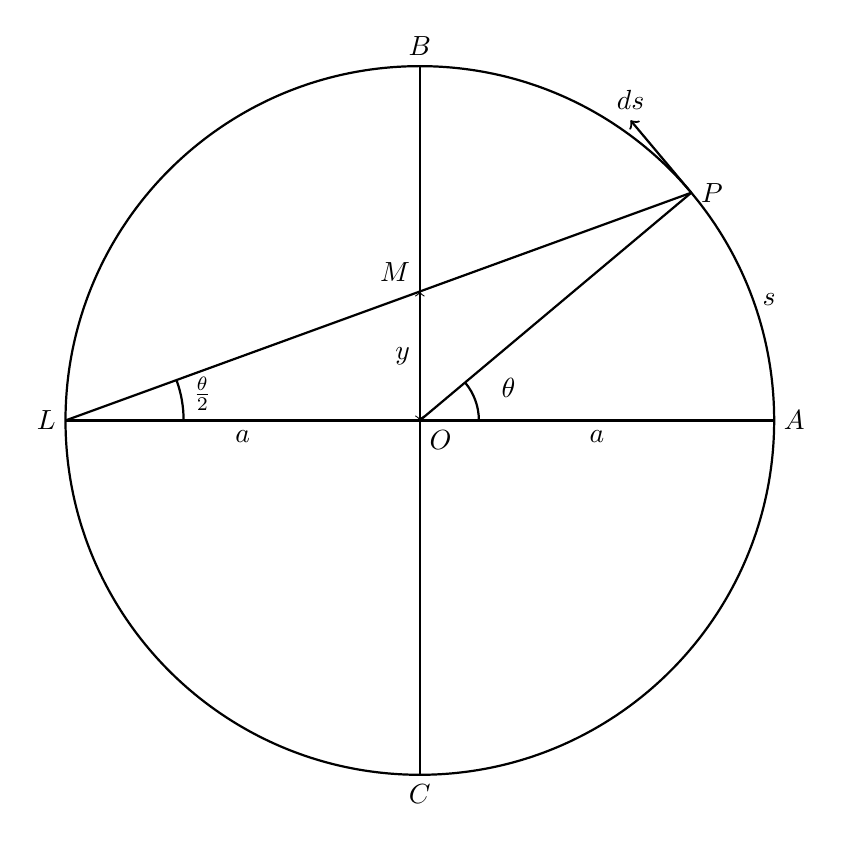
\begin{tikzpicture}[scale=1.5]
        % Draw the circle (courtyard wall)
        \draw[thick] (0,0) circle (3);
        
        % Draw the diameters
        \draw[thick] (0,-3) -- (0,3) node[above] {$B$};
        \draw[thick] (-3,0) -- (3,0);
        
        % Label key points
        \node[below] at (0,-3) {$C$};
        \node[left] at (-3,0) {$L$};
        \node[right] at (3,0) {$A$};
        
        % Add point M (man's position) and P (shadow)
        \coordinate (M) at (0,{3*tan(20)});
        \node[above left] at (M) {$M$};
        
        % Calculate P position based on similar triangles
        \coordinate (P) at ({3*cos(40)},{3*sin(40)});
        \node[right] at (P) {$P$};
        
        % Draw line from L to M and extend to P
        %\draw[dashed] (0,-3) -- (M);
        \draw[thick] (-3,0) -- (P);
        \draw[thick] (0,0) -- (P);
        
        % Draw arc s and ds
        %\draw[thick] (3,0) arc (0,18:3);
        %\draw[->,thick] (2.8,1) -- +(0.3,0.1) node[right] {$ds$};
        
        % Label arc s
        \node[right] at ({3*cos(20)},{3*sin(20)}) {$s$};
        
        % Label center
        \node[below right] at (0,0) {$O$};
        
        % Label y
        \draw[<->] (0,0.0) -- (M) node[midway,left] {$y$};
        
        % Draw angle arc and label for theta at O
        \draw[thick] (0,0) + (0:0.5) arc (0:40:0.5);
        \node at ({0.8*cos(20)},{0.8*sin(20)}) {$\theta$};
        
        % Draw angle arc and label for theta/2 at L
        \draw[thick] (-2.0,0) arc (0:20:1.0);
        \node[above right] at (-2,0) {$\frac{\theta}{2}$};
        
        % Draw tangential vector at P, anti-clockwise, and label ds
        \draw[->,thick] ({3*cos(40)},{3*sin(40)}) -- ++({130}:0.8) node[above] {$ds$};
        
        % Label radius OL with a
        \node[below] at (-1.5,0) {$a$};
        % Label radius OA with a
        \node[below] at (1.5,0) {$a$};
    \end{tikzpicture}
    \caption{Shadow cast by a moving person in a circular courtyard.}
    \label{fig:courtyard}
\end{figure}

\noindent\textbf{Solution.} In \autoref{fig:courtyard} let CB be the path of the man, and L the position of the lamp. Let M represent the position of the man at any particular instant and $y$ his distance from the center O. Then P is the position of the shadow on the circular wall and $s$ its distance AP along the curved wall from A, $ds$ being the differential of $s$ in the momentary direction of the tangent, which is continually changing so as to follow the curve, as described in article 2. In order to find the rate of the shadow $ds/dt$, when that of the man $dy/dt$, is known we must as usual find the relation between $y$ and $s$.

Draw OP and, as in \autoref{fig:courtyard}, let angle $AOP=\theta$, arc $AP=s$. Also let the radius $OL=OA=a$; $ds$ is indicated by the arrow. If a line were drawn from the end of this arrow to L, the distance between the point where it crosses OB and the point M would be $dy$, the change in $y$ corresponding to $ds$; and if a line were drawn from O to the end of the arrow, the angle between this line and OP would be $d\theta$, the change in $\theta$ corresponding to $ds$.

Using the notation just stated, we have as in \autoref{fig:courtyard}
\begin{equation}
s = a\theta \tag{a}
\end{equation}

Also, by geometry, the angle $PLA=\frac{1}{2}$(angle $POA$), or angle $MLO=\frac{\theta}{2}$ and in the right triangle MOL
\begin{equation}
y = a\tan(\theta/2) \tag{b}
\end{equation}

Differentiating (b) and (a),
\begin{align*}
dy &= a\cdot d[\tan(\theta/2)] = a\sec^2(\theta/2)\cdot d(\theta/2) \\
dy &= (a/2)\sec^2(\theta/2)\,d\theta; \quad ds = a\,d\theta
\end{align*}

From the first of these results, $d\theta = \frac{1}{(a/2)\sec^2(\theta/2)}\,dy$, and this value of $d\theta$ in the second gives
\begin{equation}
ds = \frac{2}{\sec^2(\theta/2)}\,dy \tag{c}
\end{equation}

Since $y$ and $a$ are known at any time, it is convenient to use $\tan\theta$ rather than the secant. In order to make the transformation we use the relation from trigonometry, $\sec^2\theta = 1 + \tan^2\theta$ for any angle. Therefore, equation (c) can be written as
\begin{equation}
ds = \frac{2}{1+\tan^2(\theta/2)}\,dy \tag{d}
\end{equation}

This gives the rate of the shadow in terms of the angle MLO and the rate of the man. Now, from the figure $\tan(\theta/2)=y/a$ and we have given $a=100$. Therefore, $\tan(\theta/2)=y/100$, also $dy/dt=5$, the rate of the man. Using these values, formula (d) becomes
\begin{equation*}
\frac{ds}{dt} = \frac{10}{1+(y/100)^2}
\end{equation*}

When the position of the man is stated, his distance $y$ from the center is known, and therefore the rate of the shadow on the wall $ds/dt$, is immediately calculated from this formula. We have three positions of the man given.

(i) When he is at the center $y=0$, hence $ds/dt=10$ ft./sec.

(ii) When he is 20 feet from the center $y=20$, then $y/100=\frac{1}{5}$, hence
\begin{equation*}
\frac{ds}{dt} = \frac{10}{1+(\frac{1}{5})^2} = 9.6\text{ ft./sec.}
\end{equation*}

(iii) When he is at the circumference $y=100$, then $y/100=1$ and $ds/dt=10/2=5$ ft./sec.

This is a very interesting application of the trigonometric differentiation formulas, as it also includes the method of circular measure of angles and arcs and a very instructive trigonometric formulation and transformation, beside the differentiation of the tangent of an angle.

\subsection*{An elliptical cam with shaft.}
\addcontentsline{toc}{subsection}{An elliptical cam with shaft.}

An elliptical cam arranged as in \autoref{fig:elliptical_cam} rotates about the focus $F$ as an axis and causes the roller at $P$ to move up and down along the line $FP$. If the diameters of the cam are six and ten inches and it rotates at the rate of 240 r.p.m., how fast is the roller moving at the moment when the long axis of the cam makes an angle of sixty degrees with the line of motion of the roller?

\begin{figure}[h]
    \centering
    \begin{tikzpicture}[scale=1.2]
        % Ellipse parameters
        \def\a{2.5} % semi-major axis
        \def\b{1.5} % semi-minor axis
        \def\angle{25} % rotation angle in degrees
        % Draw rotated ellipse
        \begin{scope}[rotate=\angle]
            \draw[thick] (0,0) ellipse ({\a} and {\b});
            % Major axis
            \draw[thick] (-\a,0) -- (\a,0);
            % Minor axis
            \draw[thick] (0,-\b) -- (0,\b);
            % Label a and b at midpoints
            \node[below right] at (\a/2,0) {$a$};
            \node[right] at (0,\b/2) {$b$};
        \end{scope}
        % Focus F (on x-axis, left of center)
        \def\c{sqrt(\a*\a-\b*\b)}
        \coordinate (F) at ({-\c*cos(\angle)},{-\c*sin(\angle)});
        \fill (F) circle (1.5pt);
        \node[below right] at (F) {$F$};
        % Point A (end of major axis)
        \coordinate (A) at ({\a*cos(\angle)},{\a*sin(\angle)});
        \node[right] at (A) {$A$};
        % Point P (on ellipse, vertical from F, adjusted height)
        \coordinate (P) at ({-\c*cos(\angle)},{-\c*sin(\angle)+\b*0.9});
        \fill (P) circle (1.5pt);
        \node[right] at (P) {$P$};
        % Draw FP
        \draw[thick] (F) -- (P);
        % Draw tangent at P (vertical line)
        \draw[thick] ({-\c*cos(\angle)},{-\c*sin(\angle)+\b*0.9-0.8}) -- ({-\c*cos(\angle)},{-\c*sin(\angle)+\b*0.9+0.8});
        % Draw angle arc and label for theta at F
        \draw[thick] (F) + (\angle:0.4) arc (\angle:{\angle+65}:0.4);
        \node at ({-\c*cos(\angle)+0.5*cos(\angle+32.5)},{-\c*sin(\angle)+0.5*sin(\angle+32.5)}) {$\theta$};
        % Label r
        \node[right] at ($ (F)!0.5!(P) $) {$r$};
    \end{tikzpicture}
    \caption{Elliptical cam rotating about focus $F$ with roller at $P$.}
    \label{fig:elliptical_cam}
\end{figure}

\textbf{Solution.}---Let $FP = r$ and angle $AFP = \theta$, and let the half of the long and short diameters respectively be $a$ and $b$. We then have given $\frac{d\theta}{dt} = 4$ rev./sec. $= 8\pi$ radians/sec., $a = 5$ in., $b = 3$ in., and are to find $\frac{dr}{dt}$ when $\theta = 60^\circ$. First we must have a relation between $r$ and $\theta$ in order to find $dr$ in terms of $\theta$ and $d\theta$. For the figure of an ellipse this is known to be
\begin{equation}
    r = \frac{b^2}{a(1 - e \cos \theta)}
    \tag{a}
\end{equation}
where
\begin{equation}
    e = \frac{\sqrt{a^2 - b^2}}{a}.
    \tag{b}
\end{equation}

In equation (a) therefore $b$ and $e$ are constants and we have to find $dr$ by differentiating (a). Writing (a) as
\[
    r = \frac{b^2}{a} \left( \frac{1}{1 - e \cos \theta} \right),
\]
\[
    dr = \frac{b^2}{a} \cdot d\left( \frac{1}{1 - e \cos \theta} \right)
\]
and by the formula for a reciprocal,
\[
    dr = \frac{b^2}{a} \left[ -\frac{d(1 - e \cos \theta)}{(1 - e \cos \theta)^2} \right]
    = \frac{b^2}{a} \left[ \frac{d(e \cos \theta)}{(1 - e \cos \theta)^2} \right]
\]
\[
    = \frac{b^2}{a} \left[ \frac{-e \sin \theta \, d\theta}{(1 - e \cos \theta)^2} \right]
\]
\[
    \frac{dr}{dt} = -\frac{b^2 e \sin \theta}{a (1 - e \cos \theta)^2} \frac{d\theta}{dt}
    \tag{c}
\]

Since $a = 5$, $b = 3$, equation (b) gives $e = \frac{4}{5}$; also, $b^2 = 9$ and $\frac{d\theta}{dt} = 8\pi$. Using these values, the cam data, (c) becomes
\[
    \frac{dr}{dt} = \frac{57.6\pi \sin\theta}{5(1 - \frac{4}{5} \cos\theta)^2}
\]

This formula gives the instantaneous rate at which the roller is moving for any particular value of the angle between its line of motion and the long axis of the cam, and as the cam rotates about $F$ the angle $\theta$ of course varies.

When $\theta = 60^\circ$, $\sin\theta = \frac{1}{2}\sqrt{3}$ and $\cos\theta = \frac{1}{2}$. At this instant
\[
    \frac{dr}{dt} = \frac{57.6\pi \times \sqrt{3}}{5(1 - \frac{4}{5} \cdot \frac{1}{2})^2}
    = -16\pi\sqrt{3}
\]
\[
    = -87.1 \text{ in./sec}
\]
\[
    \frac{dr}{dt} = -7.25 \text{ ft./sec}
\]

the negative sign indicating that $r$ is decreasing, and therefore the roller is moving downward.

For other values of $\theta$, that is, at other particular instants, the rate may be positive or negative, depending on the signs of the sine and cosine of the angle, for of course the roller will move both upward and downward in turn.

\section*{Exercises}
\addcontentsline{toc}{subsection}{Exercises}

\textbf{Find the differential of each of the following expressions:}

\begin{enumerate}
    \item $\sin 2x + 2\sin x$
    \item $\cos^2 x + \sin^3 x$
    \item $\cos^3 x + \cos x^3$
    \item $\cos \sqrt{1-t}$
    \item $\sin x \cdot \cos x$
    \item $x\sin x$
    \item $\frac{\theta}{2} \cos 2\theta$
    \item $\frac{1}{4} \tan 2x \cot 2x$
\end{enumerate}

\textbf{Find the derivative of each of the following expressions:}

\begin{enumerate}
    \setcounter{enumi}{8}
    \item $\dfrac{\cos x}{x}$
    \item $\sin x \cdot \sin 2x$
    \item $\sqrt{\sec 2x}$
    \item $\frac{1}{4} \tan^3 x - \tan x + x$
    \item $\frac{1 + \cos x}{1 - \cos x}$
    \item $\sin(x+a)\cos(x-a)$, $a$ constant
\end{enumerate}

\textbf{Formulate each of the following problems and solve.}

\begin{enumerate}
    \setcounter{enumi}{14}
    \item A person is approaching a 500-foot tower on a trolley car at the rate of ten miles per hour and looking at the top of the tower. At what rate must he be raising his head (or line of sight) when the car is 500 feet from the tower on level ground?\\
    (Hint: Draw a figure, call base line $x$, angle between $x$ and line of sight $\theta$, and find $d\theta/dt$ in radians and degrees per second, decreasing.)
    \item A signal observation station sights on a balloon which is rising steadily in a vertical line a mile away. At the moment when the angle of elevation of the telescope is $30^\circ$ and increasing at the rate of $1$ radian per minute, how high is the balloon and how fast is it rising?
    \item A high-speed motor torpedo boat is moving parallel to a straight shore line at 40 land miles per hour, 1.5 miles from the shore, and is followed by a search-light beam which is trained on the boat from a station half a mile back from the shore. At what rate in radians per minute must the beam turn in order to follow the boat just as the boat passes directly opposite the station, and also when it is half a mile farther along the shore past the station?
    \item A fighter plane is travelling at 300 miles per hour in a horizontal straight line and passes an enemy plane travelling in a parallel line at the same level at 250 miles per hour in the same direction. A gunner in the bomber trains his machine gun on the enemy plane as soon as he comes in range and turns the gun to keep his sights on the plane as he passes while firing on it. If the courses of the two planes are 200 yards apart, how rapidly must the machine gun be turned to follow the enemy plane just as they pass, and also half a minute afterwards?
    \item If $f = 2\sin \theta - \cos 2\theta$, is $f$ an increasing or decreasing function of $\theta$ when $\theta=45^\circ$ and when $\theta=150^\circ$? What is the rate of increase in each case, if $\theta$ is increasing at the rate of 1 radian per minute?
    \item The turning effect of a ship's rudder is shown in the theory of naval engineering to be $T= k \cos \theta \sin^2 \theta$, where $\theta$ is the angle which the rudder makes with the keel line of the ship. When the rudder is turning at $1$ radian per minute, what is the rate at which $T$ is changing, in terms of the constant $k$, at the moment when $\theta=30^\circ$?
\end{enumerate}
